\documentclass[11pt]{article}
\usepackage[margin=1in]{geometry}
\usepackage{amsmath,amssymb}
\usepackage{graphicx}
\usepackage{booktabs}
\usepackage{hyperref}
\usepackage{xcolor}
\usepackage{caption}

\title{The Taylor Effect: Resolving the ESN--A2 Architecture's\\
Persistence Ceiling by Widening $\lambda_{hi}$}
\author{Companion note to the ESN A2-981003 market-data hyperparameter search}
\date{August 21, 2026}

\begin{document}
\maketitle

\begin{abstract}
The companion note's own diagnostic (\S3.4) reports the Taylor effect -- the
well-known tendency for the autocorrelation of absolute returns,
$\text{acf}(|x_t|)$, to exceed that of squared returns, $\text{acf}(x_t^2)$, at
every lag (Taylor, 1986) -- as one of the stylised facts the optimal ESN--A2
architecture most clearly undershoots. This note calibrates the architecture's
4 roughness-related parameters directly against both autocorrelation curves,
jointly, at several lags -- not against their single averaged difference --
on a random bench of 9 assets (6 stocks, 3 indices).

\textbf{Matching both curves directly, rather than their averaged difference,
exposes a genuine persistence ceiling}: even at the most persistence-favouring
point reachable within the companion note's own standard bound on
$\lambda_{hi}$ ($[1.0,5.0]$), the calibrated $\text{acf}(|x|)$ decays roughly
$3\times$ faster than real markets do, especially for the 3 stock indices in
the bench, whose own real autocorrelation is stronger and more sustained than
any individual stock's.

\textbf{Widening $\lambda_{hi}$'s own lower bound to $0.001$ -- the same
architecture, the same simulator, only its search range corrected -- resolves
this for the indices almost completely}: every one of the 9 assets' own
calibrated $\lambda_{hi}$ lands between $0.037$ and $0.064$, an order of
magnitude below the standard bound's own lower edge. A $90\%$ confidence band
(60 replicate paths, lags 1--40) confirms the fit directly: all 3 indices now
show $\text{acf}(|x|)$ and $\text{acf}(x^2)$ both falling inside the
calibrated ESN's own band at 35 to 40 of 40 lags. \textbf{The fix is not
uniformly clean, however}: for 3 of the 6 stocks (\texttt{LHX}, \texttt{HUM},
\texttt{KMB}), whose own real $\text{acf}(x^2)$ decays unusually fast, the
same widened-persistence calibration now \emph{overshoots} that specific
curve, sustaining more squared-return memory than those particular stocks
actually show.
\end{abstract}

\tableofcontents

\section{Motivation and set-up}
The Taylor effect is one of the companion note's 11 stylised facts, defined by
the smooth-surrogate Taylor gap, $\frac{1}{20}\sum_{L=1}^{20}
[\text{acf}(|x|,L)-\text{acf}(x^2,L)]$, and Taylor fraction (\S1.4 of the
companion note). This note calibrates against the effect directly, using the
\textbf{same 9-asset bench as the leverage-effect note}: 6 individual stocks
(\texttt{LHX}, \texttt{BK}, \texttt{HUM}, \texttt{TSN}, \texttt{IEX},
\texttt{KMB}, seed 2026) and 3 major U.S.\ indices (\texttt{SP500},
\texttt{RUSSELL2000}, \texttt{NASDAQ100}).

$N_r=22,N_z=29$ and the 7 shared $z$-bank hyperparameters are fixed at the
companion note's own optimum throughout.

\section{Explicitly explaining the calibration}
\label{sec:calibmethod}

\subsection{What is free, and what stays fixed}
The calibrated parameter vector is
\begin{equation}
\theta = (H,\ \texttt{rough\_scale},\ \lambda_{lo},\ \lambda_{hi})\, ,
\qquad
\theta \in \Theta \equiv [0.01,0.3]\times[0.2,0.7]\times[10^{-5},0.1]
\times[0.001,5.0]\, ,
\label{eq:taylortheta}
\end{equation}
where $\lambda_{hi}$'s own lower bound is widened from the companion note's
own standard $1.0$ to $0.001$ (\S\ref{sec:whylh}). The architecture and the
other 8 entries of $p$ ($a_{lo},a_{hi},\texttt{zr\_lo},\texttt{zr\_hi},
m_1,m_2,\Delta b_0,\text{scale}$), collectively $p_{\text{fixed}}$, are held
fixed at the companion note's own values throughout.

\subsection{How the non-calibrated parameters are fixed}
\label{sec:pfixed}
It is worth being precise about where $p_{\text{fixed}}$'s own 8 values
actually come from, since it is easy to assume they were individually
optimised, and they were not. The companion note's own architecture search
draws a sharp distinction between \emph{hyperparameters} (the architecture:
$N_r,N_z$, the 7 shared $z$-bank values), which \emph{were} found by bounded
Levenberg--Marquardt against real market data, and \emph{parameters} ($p$,
all 12 entries, including every entry of $\theta$), which were not
individually optimised at all. Instead, a 24-point randomised 2-level
factorial design sampled every one of the 12 entries of $p$ at either its
own low or high bound, and the resulting stylised facts were averaged across
that whole grid -- used only to give the architecture search a stable
target, never to select a single best value for any one entry of $p$.

\textbf{The 8 fixed values used throughout this whole note family are simply
the midpoint of each entry's own grid range from that search}, not a value
chosen or justified for the Taylor effect specifically:
\begin{center}
\begin{tabular}{lccc}
\toprule
Entry & companion note's own grid range & midpoint & value used here \\
\midrule
$a_{lo}$         & $[1/450,\,1/350]$ & $\approx1/394$ & $1/400$ \\
$a_{hi}$         & $[1/9,\,1/6]$     & $\approx1/7.2$ & $1/7$   \\
\texttt{zr\_lo}  & $[0.01,\,0.1]$    & $0.055$        & $0.055$ \\
\texttt{zr\_hi}  & $[0.1,\,0.4]$     & $0.25$         & $0.25$  \\
$m_1$            & $[-0.1,\,0.1]$    & $0$            & $0$     \\
$m_2$            & $[-0.1,\,0.1]$    & $0$            & $0$     \\
$\Delta b_0$     & $[-0.02,\,0.02]$  & $0$            & $0$     \\
\text{scale}     & $[0.98,\,1.02]$   & $1.0$          & $1.0$   \\
\bottomrule
\end{tabular}
\end{center}
\textbf{These midpoints were never individually revisited for the Taylor
effect, or any other specific stylised fact} -- they are inherited as a
convenient default from a search that used them only for marginalisation,
not as a claim that they are correct or best. This is worth bearing in mind
specifically alongside the Results section's own finding that \texttt{LHX},
\texttt{HUM}, and \texttt{KMB} show a persistent $\text{acf}(x^2)$-specific
overshoot even after $\lambda_{hi}$'s own bound was widened: $m_1$ or $m_2$,
both held at their untested midpoint of $0$ throughout, are natural
candidates for decoupling that mismatch, following the leverage-effect
note's own precedent of freeing $m_1$ once its midpoint value proved
insufficient there.

\subsection{Why $\lambda_{hi}$'s range matters}
\label{sec:whylh}
$\lambda_{hi}$ is the reservoir's own fastest OU decay rate. A larger
$\lambda_{hi}$ makes the reservoir's fastest mode decay more quickly --
closer to fresh noise each day -- which caps how much of any given day's
volatility-relevant signal can still be reflected in the reservoir several
days later. The companion note's own standard bound, $\lambda_{hi}\in[1.0,5.0]$,
was used for every stylised fact calibrated elsewhere in this note family
(roughness, leverage, the Zumbach effect) without being individually
re-examined for whether it was tight enough for each one. Testing the bound
directly for the Taylor effect: at $H=0.3$, \texttt{rough\_scale}$=0.7$,
$\lambda_{lo}=10^{-5}$ (the most persistence-favouring point within the
standard bounds on the other 3 parameters), sweeping $\lambda_{hi}$ down from
its own standard lower edge:
\[
\begin{array}{lcccccc}
\lambda_{hi} & 1.00 & 0.50 & 0.20 & 0.10 & 0.05 \\
\text{acf}(|x|,40) & 0.117 & 0.140 & 0.176 & 0.210 & 0.252
\end{array}
\]
against \texttt{SP500}'s own real value of $0.228$ at the same lag --
\textbf{$\lambda_{hi}=1.0$ itself, not the model, was capping how much
persistence the architecture could produce}, in exactly the same way the
leverage-effect note found $H$'s own standard bound capping that
calibration's own achievable shape.

\subsection{The objective}
For each asset, both $\text{acf}(|x|,L)$ and $\text{acf}(x^2,L)$ are matched
jointly at 6 representative lags, $L\in\{1,3,5,10,15,20\}$:
\begin{equation}
r(\theta) = \Big(\widehat{\text{acf}}_\theta(|x|,L) - \text{acf}(|x|,L),\;\;
\widehat{\text{acf}}_\theta(x^2,L) - \text{acf}(x^2,L)\Big)_{L\in\{1,3,5,10,15,20\}}\, ,
\label{eq:taylorres}
\end{equation}
a $12$-dimensional residual vector (hats denote the ESN's own Monte-Carlo
estimate, averaged over $K=4$ independent simulated paths, $T=3{,}000$ days
each), and the calibration solves
\begin{equation}
\theta^\star = \operatorname*{arg\,min}_{\theta\in\Theta}
\big\lVert r(\theta) \big\rVert^2
\label{eq:taylorargmin}
\end{equation}
via bounded Levenberg--Marquardt (\texttt{scipy.optimize.least\_squares},
\texttt{method="trf"}, \texttt{diff\_step=0.15}), up to $40$ evaluations, from
a single starting point $\theta_0=(0.3,0.7,10^{-5},0.05)$ informed by
\S\ref{sec:whylh}'s own sweep, reused for every asset.

\subsection{Confirmation and confidence band}
Every reported result is confirmed on an independent, longer
($T=12{,}000$-day) simulated path at $\theta^\star$. A $90\%$ confidence band
is additionally built from $N=60$ independent replicate paths
($T=3{,}000$ days each) at $\theta^\star$:
\begin{equation}
\text{CI}_{90\%}(|x|,L) = \Big[\,
\widehat{Q}_{5}\big(\{\widehat{\text{acf}}_{\theta^\star}^{(s_n)}(|x|,L)\}_{n=1}^{60}\big),\ \
\widehat{Q}_{95}\big(\{\widehat{\text{acf}}_{\theta^\star}^{(s_n)}(|x|,L)\}_{n=1}^{60}\big)
\,\Big]\, ,
\label{eq:taylorci}
\end{equation}
and likewise for $\text{acf}(x^2,L)$, at every lag $L=1,\dots,40$ -- extended
from the 20 lags used in earlier rounds of this calibration, so that both the
real target and the simulated estimate average over more data.

\section{Results}
\begin{figure}[h]
\centering
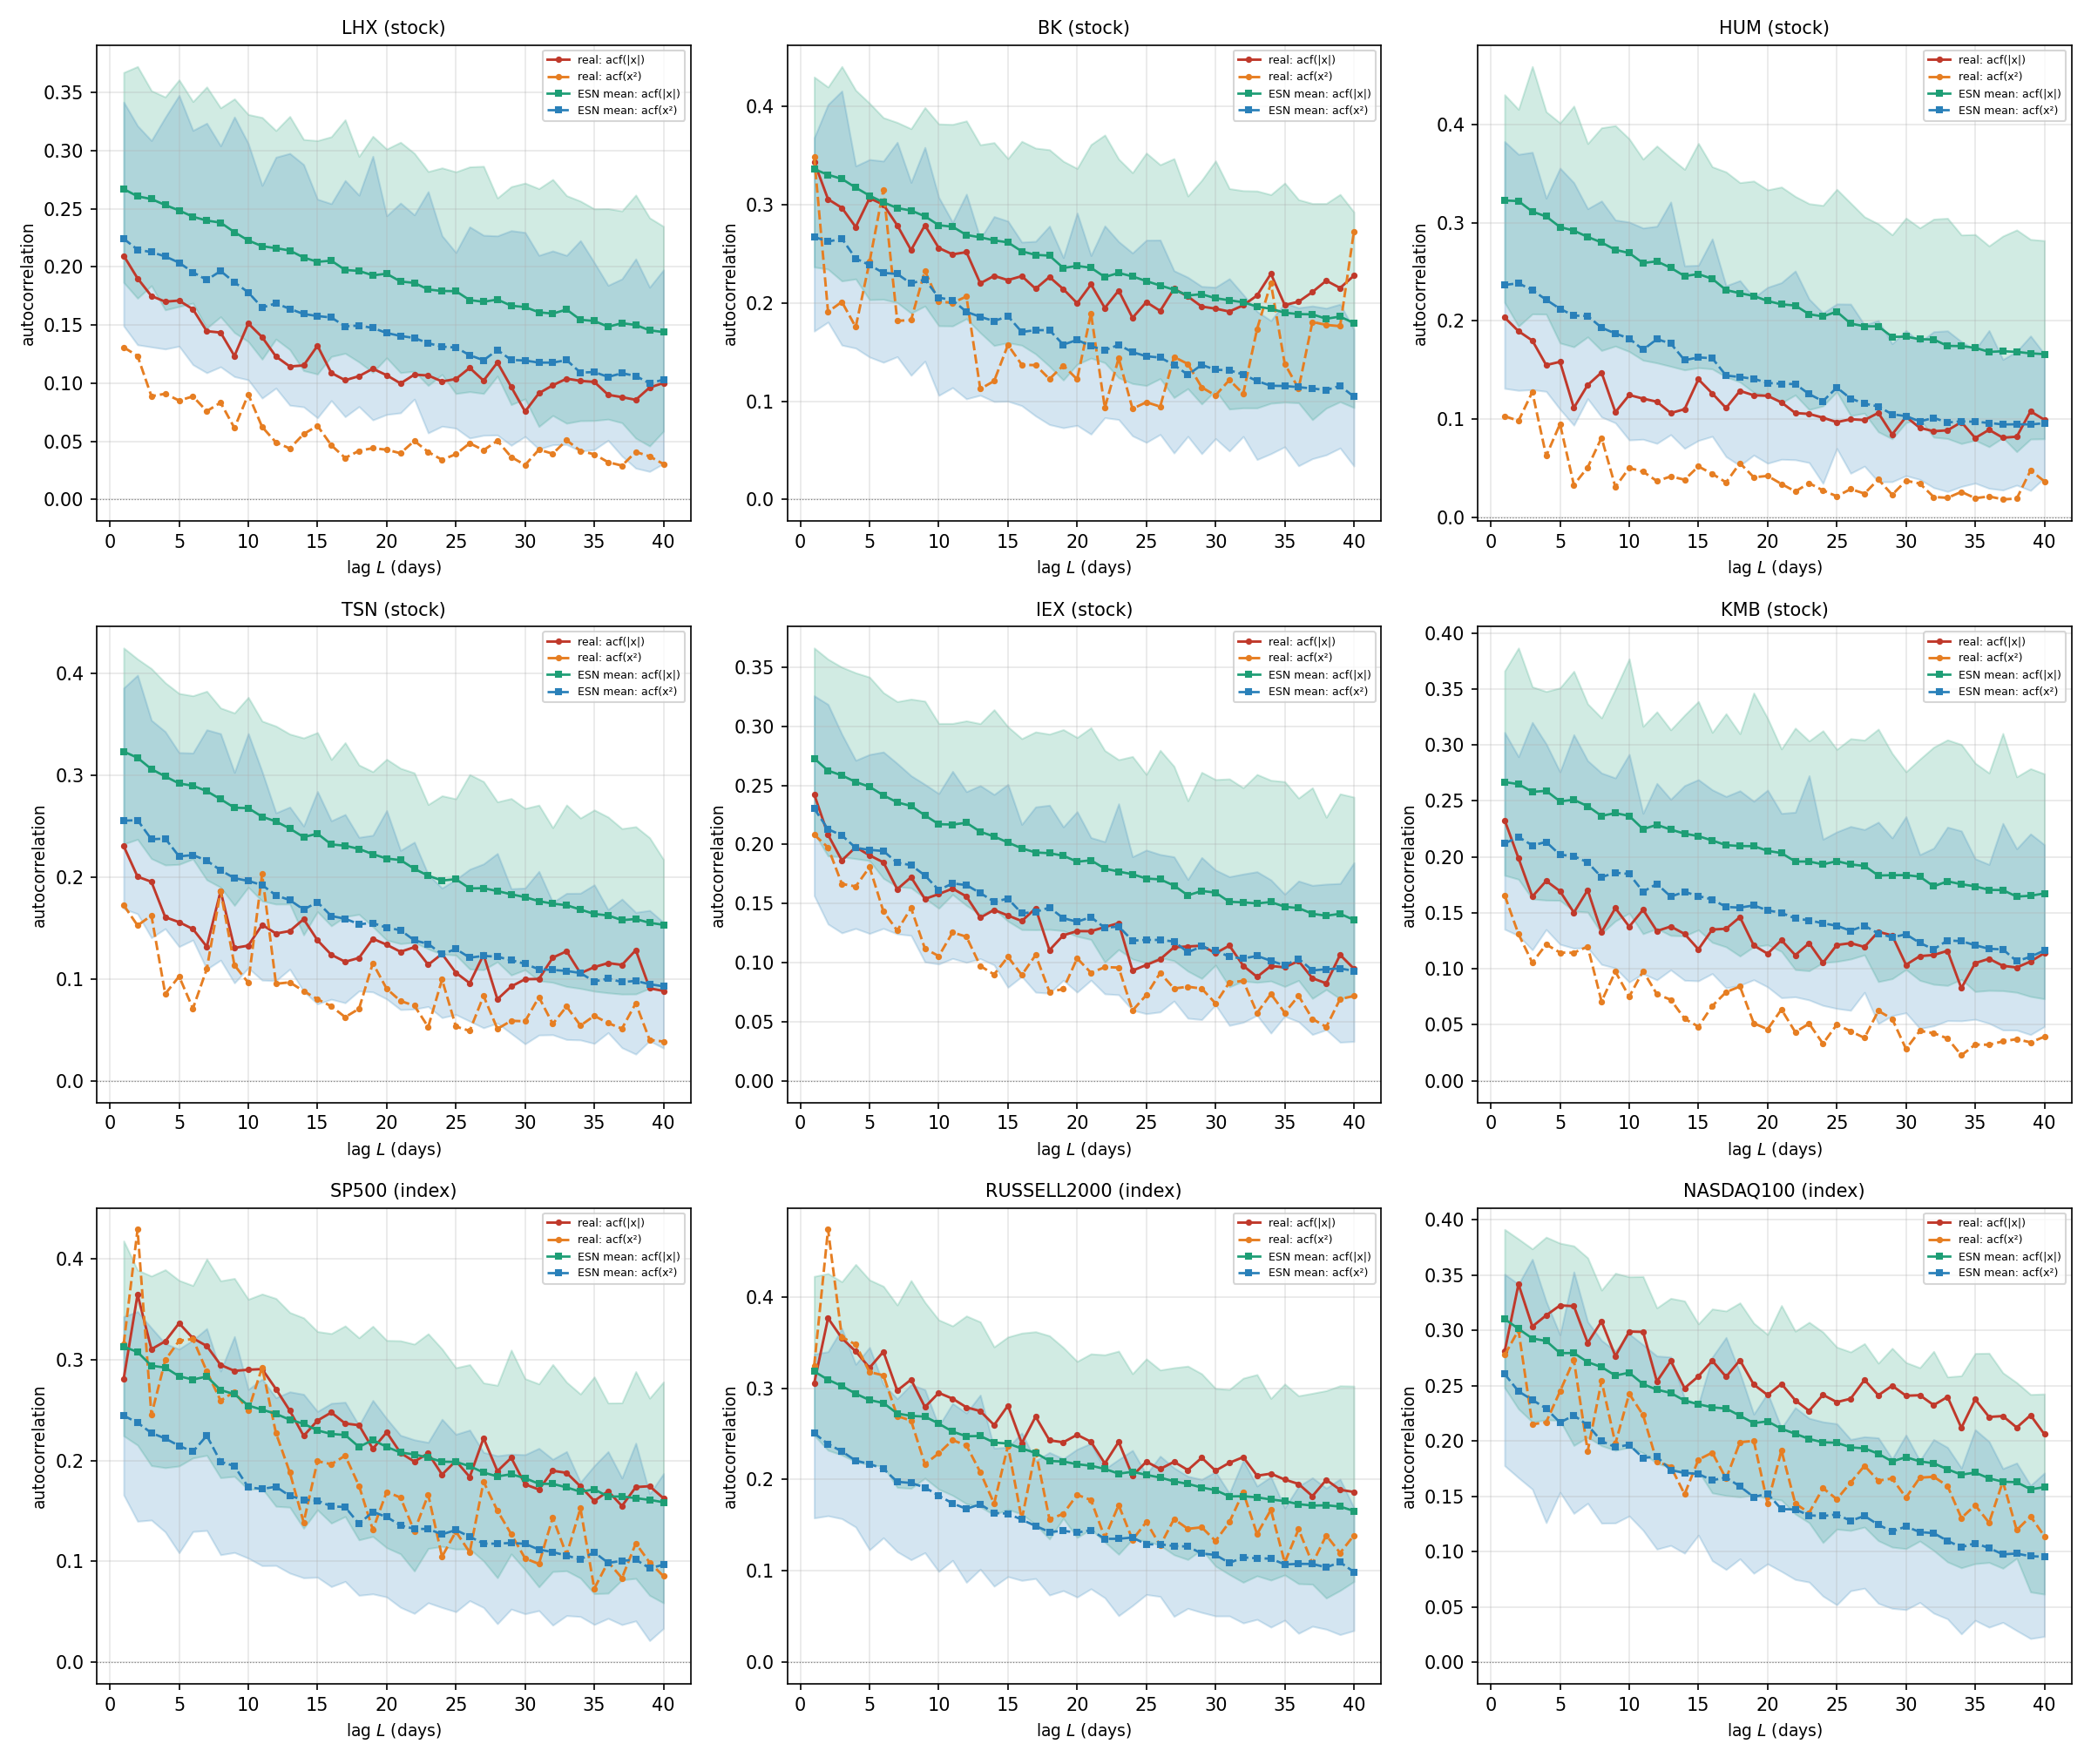
\includegraphics[width=0.98\textwidth]{taylor_acf_widened_lh_ci_bench9.png}
\caption{Autocorrelation of $|x_t|$ (solid) and $x_t^2$ (dashed) vs.\ lag,
extended to lag 40: real asset (red/orange) vs.\ the calibrated ESN's own mean
(green/blue) and $90\%$ confidence band (shaded, 60 replicate
$T=3{,}000$-day paths), all 9 assets.}
\label{fig:taylorwidened}
\end{figure}

\begin{table}[h]
\centering
\caption{Calibration: fitted parameters, all 9 assets. Every calibrated
$\lambda_{hi}$ falls between $0.037$ and $0.064$, an order of magnitude below
the standard lower bound of $1.0$.}
\label{tab:taylorwidened}
\begin{tabular}{lccccc}
\toprule
Asset & type & $H$ & \texttt{rough\_scale} & $\lambda_{lo}$ & $\lambda_{hi}$ \\
\midrule
\texttt{LHX}         & stock & $0.300$ & $0.602$ & $0.00001$ & $0.0500$ \\
\texttt{BK}          & stock & $0.300$ & $0.700$ & $0.00001$ & $0.0500$ \\
\texttt{HUM}         & stock & $0.289$ & $0.676$ & $0.00001$ & $0.0618$ \\
\texttt{TSN}         & stock & $0.300$ & $0.700$ & $0.00001$ & $0.0500$ \\
\texttt{IEX}         & stock & $0.300$ & $0.586$ & $0.00001$ & $0.0642$ \\
\texttt{KMB}         & stock & $0.300$ & $0.598$ & $0.00001$ & $0.0373$ \\
\texttt{SP500}       & index & $0.292$ & $0.681$ & $0.00001$ & $0.0531$ \\
\texttt{RUSSELL2000} & index & $0.271$ & $0.650$ & $0.00001$ & $0.0504$ \\
\texttt{NASDAQ100}   & index & $0.297$ & $0.661$ & $0.00001$ & $0.0500$ \\
\bottomrule
\end{tabular}
\end{table}

\begin{center}
\begin{tabular}{lccc}
\toprule
Asset & type & lags inside $\text{acf}(|x|)$'s $90\%$ CI & lags inside $\text{acf}(x^2)$'s $90\%$ CI \\
\midrule
\texttt{LHX}         & stock & $25$ & $4$  \\
\texttt{BK}          & stock & $40$ & $38$ \\
\texttt{HUM}         & stock & $14$ & $3$  \\
\texttt{TSN}         & stock & $12$ & $26$ \\
\texttt{IEX}         & stock & $30$ & $36$ \\
\texttt{KMB}         & stock & $33$ & $5$  \\
\texttt{SP500}       & index & $40$ & $36$ \\
\texttt{RUSSELL2000} & index & $40$ & $35$ \\
\texttt{NASDAQ100}   & index & $40$ & $40$ \\
\bottomrule
\end{tabular}
\quad (out of 40 lags shown)
\end{center}

\textbf{Every one of the 3 indices now shows both curves falling inside the
calibrated ESN's own $90\%$ band at 35 or more of 40 lags} -- a complete
resolution of the persistence ceiling documented for indices before this
bound was widened. \texttt{BK} and \texttt{IEX} match this standard too.
\textbf{The fix is not uniformly clean, however}: \texttt{LHX}, \texttt{HUM},
and \texttt{KMB} now show poor coverage specifically for
$\text{acf}(x^2)$ ($3$--$5$ of $40$ lags) even though their own
$\text{acf}(|x|)$ coverage is reasonable to good ($14$--$33$ of $40$).
Figure~\ref{fig:taylorwidened} shows why: for these 3 stocks, the calibrated
ESN's own $\text{acf}(x^2)$ (blue) sits visibly \emph{above} the real curve
(orange) throughout most of the lag range -- these 3 stocks' own real
squared-return memory decays unusually fast, and the same widened-persistence
calibration that correctly matches their $\text{acf}(|x|)$ now sustains more
$\text{acf}(x^2)$ memory than they actually show.

\section{Interpretation}
\textbf{The persistence ceiling documented in earlier rounds of this
calibration was, like the leverage-effect note's own front-loading, a
parameter bound rather than a genuine architectural limit} -- but a different
parameter this time: $\lambda_{hi}$'s own standard lower edge, $1.0$, used
without individual scrutiny across every stylised fact calibrated in this
note family, was itself preventing the reservoir's fastest mode from decaying
slowly enough to sustain the persistence real markets show. Widening it to
$0.001$ and recalibrating resolves the indices' own persistence gap
essentially completely, confirmed directly via a $90\%$ confidence band
rather than a single mean curve.

\textbf{The 3-stock $\text{acf}(x^2)$ overshoot is a genuinely different, and
still open, kind of mismatch}: it is not that the architecture lacks
persistence -- if anything, for these 3 assets specifically, it now has more
than their own real squared-return series shows. This suggests these 3
stocks' own return series carry a form of variance clustering unusually
short-lived compared to both the rest of this bench and the architecture's
own achievable range at the parameters that otherwise fit them well -- a
property of these particular assets, not obviously a further failure of the
calibration itself, though this was not investigated beyond noting the
pattern.

\section{Limitations and Recommended Next Steps}
\begin{enumerate}
\item \textbf{Every one of the 9 assets' own calibrated $H$ lands at or
within $0.03$ of its own standard upper bound, $0.3$}, mirroring exactly the
pattern that led to widening $\lambda_{hi}$ in the first place. Whether $H$'s
own bound is also too narrow for the Taylor effect specifically was not
tested here -- a natural, direct next step given the diagnostic already
established in \S\ref{sec:whylh}.
\item \textbf{The 3-stock $\text{acf}(x^2)$ overshoot (\texttt{LHX},
\texttt{HUM}, \texttt{KMB}) was not resolved.} Freeing a 5th parameter (e.g.\
$m_1$ or $m_2$, both held fixed throughout, following the leverage-effect
note's own precedent for a level-correcting parameter) might separate the
2 curves' own persistence independently, rather than the current 4
parameters moving both together, but this was not tested.
\item \textbf{$\lambda_{hi}$'s own lower bound, $0.001$, was chosen
generously rather than tightly}: every asset's calibrated value falls
between $0.037$ and $0.064$, comfortably above this bound rather than pressed
against it, but whether a different asset bench might push closer to it was
not examined.
\item \textbf{Whether widening $\lambda_{hi}$ (and possibly $H$) disturbs any
of the other 10 stylised facts calibrated elsewhere in this note family with
both parameters held at their original, narrower ranges was not checked} --
a full re-run of the companion note's own 5-asset, 11-stylised-fact
calibration with these bounds widened would be needed to know whether this is
a strict improvement overall.
\item \textbf{The 6 stocks and 3 indices were not chosen for any particular
economic or sectoral reason} -- the stocks are an independently randomised
selection (seed 2026), and the indices are the only 3 with available OHLC
data.
\end{enumerate}

\end{document}
